% Compile with xelatex (the Chinese text needs xeCJK and a CJK font). Figures are the vector PDFs in
% paper/figures/out; the references are already formatted (citeproc), so no BibTeX run is needed.
% Options for packages loaded elsewhere
\PassOptionsToPackage{unicode}{hyperref}
\PassOptionsToPackage{hyphens}{url}
\PassOptionsToPackage{space}{xeCJK}
%
\documentclass[
]{article}
\usepackage{amsmath,amssymb}
\usepackage{iftex}
\ifPDFTeX
  \usepackage[T1]{fontenc}
  \usepackage[utf8]{inputenc}
  \usepackage{textcomp} % provide euro and other symbols
\else % if luatex or xetex
  \usepackage{unicode-math} % this also loads fontspec
  \defaultfontfeatures{Scale=MatchLowercase}
  \defaultfontfeatures[\rmfamily]{Ligatures=TeX,Scale=1}
\fi
\usepackage{lmodern}
\ifPDFTeX\else
  % xetex/luatex font selection
  \setmainfont[]{TeX Gyre Termes}
  \ifXeTeX
    \usepackage{xeCJK}
    \setCJKmainfont[]{Noto Serif CJK SC}
          \fi
  \ifLuaTeX
    \usepackage[]{luatexja-fontspec}
    \setmainjfont[]{Noto Serif CJK SC}
  \fi
\fi
% Use upquote if available, for straight quotes in verbatim environments
\IfFileExists{upquote.sty}{\usepackage{upquote}}{}
\IfFileExists{microtype.sty}{% use microtype if available
  \usepackage[]{microtype}
  \UseMicrotypeSet[protrusion]{basicmath} % disable protrusion for tt fonts
}{}
\makeatletter
\@ifundefined{KOMAClassName}{% if non-KOMA class
  \IfFileExists{parskip.sty}{%
    \usepackage{parskip}
  }{% else
    \setlength{\parindent}{0pt}
    \setlength{\parskip}{6pt plus 2pt minus 1pt}}
}{% if KOMA class
  \KOMAoptions{parskip=half}}
\makeatother
\usepackage{xcolor}
\usepackage[margin=2.5cm]{geometry}
\usepackage{longtable,booktabs,array}
\usepackage{calc} % for calculating minipage widths
% Correct order of tables after \paragraph or \subparagraph
\usepackage{etoolbox}
\makeatletter
\patchcmd\longtable{\par}{\if@noskipsec\mbox{}\fi\par}{}{}
\makeatother
% Allow footnotes in longtable head/foot
\IfFileExists{footnotehyper.sty}{\usepackage{footnotehyper}}{\usepackage{footnote}}
\makesavenoteenv{longtable}
\usepackage{graphicx}
\makeatletter
\def\maxwidth{\ifdim\Gin@nat@width>\linewidth\linewidth\else\Gin@nat@width\fi}
\def\maxheight{\ifdim\Gin@nat@height>\textheight\textheight\else\Gin@nat@height\fi}
\makeatother
% Scale images if necessary, so that they will not overflow the page
% margins by default, and it is still possible to overwrite the defaults
% using explicit options in \includegraphics[width, height, ...]{}
\setkeys{Gin}{width=\maxwidth,height=\maxheight,keepaspectratio}
% Set default figure placement to htbp
\makeatletter
\def\fps@figure{htbp}
\makeatother
\setlength{\emergencystretch}{3em} % prevent overfull lines
\providecommand{\tightlist}{%
  \setlength{\itemsep}{0pt}\setlength{\parskip}{0pt}}
\setcounter{secnumdepth}{5}
\newlength{\cslhangindent}
\setlength{\cslhangindent}{1.5em}
\newlength{\csllabelwidth}
\setlength{\csllabelwidth}{3em}
\newlength{\cslentryspacingunit} % times entry-spacing
\setlength{\cslentryspacingunit}{\parskip}
\newenvironment{CSLReferences}[2] % #1 hanging-ident, #2 entry spacing
 {% don't indent paragraphs
  \setlength{\parindent}{0pt}
  % turn on hanging indent if param 1 is 1
  \ifodd #1
  \let\oldpar\par
  \def\par{\hangindent=\cslhangindent\oldpar}
  \fi
  % set entry spacing
  \setlength{\parskip}{#2\cslentryspacingunit}
 }%
 {}
\usepackage{calc}
\newcommand{\CSLBlock}[1]{#1\hfill\break}
\newcommand{\CSLLeftMargin}[1]{\parbox[t]{\csllabelwidth}{#1}}
\newcommand{\CSLRightInline}[1]{\parbox[t]{\linewidth - \csllabelwidth}{#1}\break}
\newcommand{\CSLIndent}[1]{\hspace{\cslhangindent}#1}
\ifLuaTeX
\usepackage[bidi=basic]{babel}
\else
\usepackage[bidi=default]{babel}
\fi
\babelprovide[main,import]{american}
\ifPDFTeX
\else
\babelfont{rm}[]{TeX Gyre Termes}
\fi
% get rid of language-specific shorthands (see #6817):
\let\LanguageShortHands\languageshorthands
\def\languageshorthands#1{}
\ifLuaTeX
  \usepackage{selnolig}  % disable illegal ligatures
\fi
\IfFileExists{bookmark.sty}{\usepackage{bookmark}}{\usepackage{hyperref}}
\IfFileExists{xurl.sty}{\usepackage{xurl}}{} % add URL line breaks if available
\urlstyle{same}
\hypersetup{
  pdftitle={TaoChronos: A Reliable Agent for Knowledge Discovery in Traditional Chinese Medicine},
  pdflang={en-US},
  hidelinks,
  pdfcreator={LaTeX via pandoc}}

\title{TaoChronos: A Reliable Agent for Knowledge Discovery in
Traditional Chinese Medicine}
\author{}
\date{}

\begin{document}
\maketitle

\textbf{Authors:} {[}Author 1{]}\textsuperscript{a,*}, {[}Author
2{]}\textsuperscript{a}, \ldots{} {[}Corresponding
author{]}\textsuperscript{a,*}

\textsuperscript{a} IMPF-AI (医哲未来人工智能研究院), {[}address{]}.
*Corresponding author. E-mail address: {[}e-mail{]}.

\textbf{Article type:} Research Article

\hypertarget{abstract}{%
\section*{Abstract}\label{abstract}}
\addcontentsline{toc}{section}{Abstract}

Large language models (LLMs) can mine the classical literature of
traditional Chinese medicine (TCM), yet what they assert may misquote
the texts, misread negations and conditions, count copies of one text as
independent testimony, equate historical with modern diseases, and
resist checking without hindsight. We present TaoChronos, an agent for
knowledge discovery from the Chinese medical classics engineered so that
reliability is a property of its architecture rather than of its model:
models and rules only propose, deterministic validators grade, and human
experts alone approve. Every state change is a typed event checked
against the authority of its emitter; every claim must quote a dated
witness verbatim and be stated by that quote; and an executable research
contract, fixed before the first task, decides acceptance. On a corpus
of 966 witnesses (123 million characters, 475 BCE--1949), TaoChronos
rejected 180 of 180 corrupted quotations, kept 19 of 19 safety
invariants, each of which broke when its safeguard was removed, and read
82 of 84 held-out hard interpretive cases correctly. In a blind temporal
benchmark, rankings from texts written before a cutoff anticipated links
later physicians wrote (precision@10 0.168 vs 0.134 for popularity and
0.054 for chance; \emph{P} = 2.4 × 10⁻¹⁶). All results were obtained
without calling a language model.

\textbf{Keywords:} Traditional Chinese medicine; Large language model
agents; Knowledge discovery; Provenance; Trustworthy artificial
intelligence

\hypertarget{introduction}{%
\section{Introduction}\label{introduction}}

The classical literature of traditional Chinese medicine (TCM) is one of
the longest written records of clinical observation, and it has yielded
medicines: a fourth-century prescription in Ge Hong's \emph{Zhouhou
beiji fang} suggested the low-temperature extraction that led to
artemisinin {[}\protect\hyperlink{ref-tu2011artemisinin}{1}{]}, and
arsenic, a mineral drug of the tradition, became a cure for acute
promyelocytic leukemia {[}\protect\hyperlink{ref-wang2008apl}{2}{]}.
Literature-based discovery joins what different texts say
{[}\protect\hyperlink{ref-swanson1986fish}{3}{]}, and machine reading of
modern literature anticipates findings before they are published
{[}\protect\hyperlink{ref-tshitoyan2019unsupervised}{4},\protect\hyperlink{ref-krenn2023forecasting}{5}{]}.
The TCM classics are harder: a passage survives in witnesses that differ
character by character, its date is often a range, commentaries
accumulated over centuries, names changed their meaning, and most of
what later books say was copied from earlier ones.

ZhongJingGPT, introduced in 2023 as the first large language model
dedicated to TCM, fine-tuned general-purpose models on instructions
constructed from TCM expert knowledge
{[}\protect\hyperlink{ref-kang2025zhongjinggpt}{6},\protect\hyperlink{ref-cmlm2023zhongjing}{7}{]};
Chinese medical models
{[}\protect\hyperlink{ref-zhang2023huatuogpt}{8},\protect\hyperlink{ref-yang2024zhongjing}{9}{]},
TCM benchmarks {[}\protect\hyperlink{ref-yue2024tcmbench}{10}{]} and
LLM-built knowledge graphs of the ancient literature
{[}\protect\hyperlink{ref-li2025tcmrdkg}{11},\protect\hyperlink{ref-xiang2025kgclassics}{12}{]}
followed. LLM agents now plan experiments and propose and test
hypotheses
{[}\protect\hyperlink{ref-boiko2023autonomous}{13}--\protect\hyperlink{ref-lu2026endtoend}{17}{]}.
In these systems reliability rests largely on the model, and LLMs can
state fluent claims with unsupported citations
{[}\protect\hyperlink{ref-ji2023hallucination}{18}--\protect\hyperlink{ref-thirunavukarasu2023llm}{20}{]}.
On historical medical texts the failure modes are specific (Table 1).

We argue that reliability must be engineered into the agent's
architecture. TaoChronos (道乃久) follows one principle,
\emph{deterministic harness, stochastic intelligence}: state,
permissions, verification, stopping and acceptance are deterministic
code, and intelligence --- a language model or a rule-based procedure
standing in for one --- may only propose. Our four contributions are:

\begin{enumerate}
\def\labelenumi{\arabic{enumi}.}
\tightlist
\item
  \textbf{An agent architecture that separates proposal from verdict:}
  an event-sourced research object, authority by principal over 61 event
  types, a permissioned tool mesh, hooks that require verbatim and
  semantically supported quotations, nine epistemic gates and an
  executable research contract (Fig. 1).
\item
  \textbf{A dated, layered and license-tracked corpus} of 966 witnesses
  of 761 works (about 123 million characters, 2.05 million passages, 475
  BCE--1949), with an openly licensed canon defined by the tradition's
  own citations that runs in a web browser (Fig. 2).
\item
  \textbf{A three-layer evaluation of reliability and research value:}
  safety invariants checked by mutation, hard interpretive cases with
  unsafe errors counted apart in blind rounds, and a blind temporal
  benchmark in which leakage is counted rather than assumed (Figs. 4 and
  5).
\item
  \textbf{Guarded ancient--modern translation and full transparency:}
  phenotypic similarity to modern diseases through the Human Phenotype
  Ontology {[}\protect\hyperlink{ref-kohler2021hpo}{21}{]}, never
  retrospective diagnosis, and a complete, replayable research run
  released with its unrepaired failure analysis (Fig. 3).
\end{enumerate}

\hypertarget{materials-and-methods}{%
\section{Materials and methods}\label{materials-and-methods}}

\hypertarget{corpus}{%
\subsection{Corpus}\label{corpus}}

Transcriptions came from ten sources, among them the Kanseki Repository
(the \emph{Siku quanshu} medical section), JiCheng (中醫笈成), CMETA
(數位中醫校書郎), Wikisource and McGill University Library
(Supplementary Table 13). Admission removes contemporary publications
and modern annotated editions; de-duplication against more trusted
sources uses normalized 12-character shingles, while independently
collated transcriptions are kept as separate witnesses. Dating is
layer-aware: main text, commentaries, editors' notes and later additions
are dated apart, from curated overrides, book records, dated prefaces
(parsed with a table of reign eras), other witnesses and the author's
life; an undatable witness is placed in the Qing (1644--1911), never
earlier. Each passage keeps its book, edition, locator, date range,
layer, transcription source and license; normalization of variant forms
is used for matching only. A work's influence is 10 log₂(1 + citing
works) + 2 × (periods citing it) + 2 log₂(1 + citations) + 3 log₂(1 +
witnesses) + 6 × (inclusion in the \emph{Siku quanshu}); the openly
licensed witnesses of the 350 highest-ranked works form the web corpus
(348 works, 368 witnesses, 8.51 million characters) used in Figs. 2e and
3.

\hypertarget{agent-architecture}{%
\subsection{Agent architecture}\label{agent-architecture}}

The research object holds all scientific state and is changed only by a
reducer applying typed events in transactions; each event carries its
principal (kernel, human, validator or agent), set from an identity
object, and the reducer refuses an event its principal may not emit
(Fig. 1b). Agents propose; only validators grade gates, scores and the
contract; only a human sets gate G7 (expert approval); an objection
closes only when a validator re-runs its check or an expert decides.
Sixteen agents (a Director and fifteen specialists, from Curator and
Philologist to Hypothesis agent and Skeptic) are configurations naming
permissions, tools, context view, output schema, model tier and budget;
a deterministic procedure and a model produce the same typed output,
verified by one commit function. Each of 73 tools needs one of seven
permissions; a scope guard and a result firewall wrap every call;
receipts form a hash chain. The state hash covers scientific fields
only, so reruns, resumed and parallel runs agree.

\hypertarget{claims-readings-discovery-and-acceptance}{%
\subsection{Claims, readings, discovery and
acceptance}\label{claims-readings-discovery-and-acceptance}}

The Extractor turns passages into claim hyperedges,
e.g.~indicated\_for(formula: 五苓散 \textbar{} pulse: 浮, symptom:
小便不利, symptom: 微热, disease: 消渴), with spans, negations and
conditions. At commit the harness relocates every quotation in its
passage and a semantic-support reader checks that the quotation states
the relation, reading cues, consequences, pronouns, negations and the
statement frame (speaker; asserted, reported or rejected stance); a
contradicted claim is refused, and a registry of textual cruxes
harvested from commentaries makes doubtful clauses read as ambiguous.
Five engines propose: lost knowledge (D1), concept drift by
Jensen--Shannon divergence with permutation tests (D2), formula
evolution (D3), hidden associations by Adamic--Adar link prediction
{[}\protect\hyperlink{ref-adamic2003friends}{22}{]} (D4) and
contradictions (D5). The Skeptic tries to refute each hypothesis
{[}\protect\hyperlink{ref-popper1959logic}{23}{]}; for arguments from
silence it searches the whole scope for explicit supported statements,
which raise hard, critical objections. Gates G0--G8 grade source,
transcription, philology, sense, claim provenance, independent source
families, falsification, expert approval and modern evidence; the
contract judges each hypothesis on its current version as accepted,
needing an expert, inconclusive or rejected.

\hypertarget{evaluation-design}{%
\subsection{Evaluation design}\label{evaluation-design}}

Forty suites form three layers (Supplementary Table 1). (i) Nineteen
invariants run as probes against the agent and against six variants,
each with one boundary deleted at run time
{[}\protect\hyperlink{ref-jia2011mutation}{24}{]}. (ii) 107 hard
interpretive cases in eight classes (23 development, 84 held out, split
fixed before the first run), unsafe errors counted apart, and four blind
rounds written before the rules that first read them. (iii) A blind
temporal benchmark: the full corpus is split at 1127 and 1368, a passage
belonging to a side only if its whole date range does, with every read
path bounded in SQL; for each disease or symptom with 150--6,000 past
and ≥ 300 future passages, unlinked formulas and drugs of its past graph
are ranked, and a candidate comes true when claims in ≥ 2 later books
link it. Precision@\emph{k} has Wilson intervals
{[}\protect\hyperlink{ref-wilson1927probable}{25}{]}, mean average
precision a 999-resample bootstrap interval, and paired comparisons
two-sided exact sign tests. Rules were written before the first run; all
results used rules only.

\hypertarget{results}{%
\section{Results}\label{results}}

\hypertarget{a-dated-layered-corpus}{%
\subsection{A dated, layered corpus}\label{a-dated-layered-corpus}}

The store holds 966 witnesses, 537 dated to a single year; the basis of
each date is recorded, from curation (329) to signed prefaces (139); 104
undated witnesses are counted as Qing (Fig. 2). Records of 10,001
printed and manuscript copies in eleven digitized collections link 179
works to physical witnesses (Supplementary Fig. 4).

\hypertarget{one-research-question-end-to-end}{%
\subsection{One research question, end to
end}\label{one-research-question-end-to-end}}

We asked how the composition and indications of Shenqi wan changed over
time, with Shenqi wan and Liuwei dihuang wan as focus terms and 消渴 =
diabetes forbidden, on the open corpus (206 books, 1,399 passages; Fig.
3a). The run planned 30 tasks in three rounds, wrote 734 events, called
156 tools (none refused) and no model; it extracted 777 claims and
recorded 87 evidence and 22 counter-evidence records (Fig. 3b). Of 14
hypotheses, the Skeptic kept 3, sent 10 to be narrowed and rejected 1,
raising 117 objections (Fig. 3c). One hypothesis (restlessness 烦躁 as
an indication of Liuwei dihuang wan) met every machine-checkable
criterion on two independent source families and awaits an expert;
twelve were inconclusive, all short of two independent families; one, a
`lost' association of Lizhong wan with fever, was rejected because a
later book restates it (Fig. 3d,e). A second run wrote the same report.

Reading every hypothesis against its evidence found five failure modes
(Supplementary Fig. 1). The independence gate merged books linked by any
transcription or rephrasing, transitively, putting 35 of the 38 evidence
books in one family; with transcription links only, five failed
hypotheses would rest on two to four families. The rules also read
co-occurrence as association, dated a commentary of 1547 with its base
text of 1237, stated one contradiction twice and, on the sampled open
corpus, missed the 1119 first record of Liuwei dihuang wan. None
concerned the hypothesis that passed, and the largest made the gate
stricter, not looser; we report them unrepaired.

\hypertarget{quotations-boundaries-and-hard-readings}{%
\subsection{Quotations, boundaries and hard
readings}\label{quotations-boundaries-and-hard-readings}}

On 60 random passages, all verbatim quotations were accepted and all 180
corrupted ones (one character replaced, random characters, shifted span)
rejected (Fig. 4a). All 19 invariants held on the intact agent; each
removed boundary broke the invariant named for it and no other (127 of
133 cells held; Fig. 4b). The agent read 82 of 84 held-out hard cases
correctly (0.976); both errors were unsafe, textual cruxes the harvest
does not find (Fig. 4c). Blind rounds scored 43/53, 30/32, 7/10 (a new
class of cruxes) and, after a registry of 127 cruxes was harvested from
the commentaries, 5/5 (Fig. 4d). On 25,000 full-corpus passages this
second reader found 71 rule claims contradicted by their own quotes;
after the extractor was fixed, the 12 left are refused at commit.

\hypertarget{rankings-from-the-past-anticipate-later-links}{%
\subsection{Rankings from the past anticipate later
links}\label{rankings-from-the-past-anticipate-later-links}}

In 189 topic--cutoff pairs with a link that came true (29,467
candidates, 1,314 true; base rate 4.5\%), Adamic--Adar reached
precision@10 0.168 (95\% CI 0.152--0.185) against 0.134 for popularity
and 0.054 for chance, and mean average precision 0.199 against 0.143 and
0.092 (Fig. 5b); it beat popularity in 149 pairs and lost in 39
(\emph{P} = 2.4 × 10⁻¹⁶; Fig. 5c). Leakage was zero. Run on the past
view at 1368, the pipeline's surviving held-out predictions were
discoveries (true and new) in 7 of 19 (0.37; 95\% CI 0.19--0.59), after
absence checks rejected two wrong `lost' and two already-written
`hidden' associations and no discovery (Fig. 5d). On the open corpus
alone (30 pairs) Adamic--Adar beat popularity (24/6, \emph{P} = 0.0014)
but not chance (13/17, \emph{P} = 0.58; Supplementary Fig. 3): the
benchmark needs the full corpus.

\hypertarget{generalization-the-study-layer-and-the-bridge}{%
\subsection{Generalization, the study layer and the
bridge}\label{generalization-the-study-layer-and-the-bridge}}

Held-out data show where rules transfer (Supplementary Fig. 2,
Supplementary Table 14): entity recognition fell from F1 0.99 to 0.78
and lost-text reconstruction from precision 0.86 to 0.32, while a
learned punctuation model reached boundary F1 0.767 on 55 held-out works
(rules 0.235) without changing a character. The deterministic study
layer recovers dated taboo renamings (薯蓣 → 山药, 1000--1200; 玄参 →
元参, 1600--1800), the Qing rise of warm disease (Cochran--Armitage
\emph{z} = 6.62 {[}\protect\hyperlink{ref-armitage1955tests}{26}{]}) and
the drug cores of classical formulas (Supplementary Fig. 5). The
ancient--modern bridge maps 168 ancient phenotypes onto 213 HPO terms
with typed relations and 64 disease profiles at qualitative levels; on
12 random held-out passages it reached F1 0.822 (precision 0.938, recall
0.732), and its presentism guard handled 24 of 24 translation cases.
Modern evidence is typed by design and population, and real-world-data
questions compile to one checked, read-only OMOP query
{[}\protect\hyperlink{ref-hripcsak2015ohdsi}{27}{]}, never model-written
SQL.

\hypertarget{discussion}{%
\section{Discussion}\label{discussion}}

TaoChronos shows that the reliability of a discovery agent can be
engineered and measured. The checks are code a model cannot route
around: a misquotation cannot be committed, an agent cannot approve its
own hypothesis, a finished run is not an accepted finding, and a test of
foresight cannot read the future; each boundary was measured by deleting
it. The design complements TCM language models such as ZhongJingGPT
{[}\protect\hyperlink{ref-kang2025zhongjinggpt}{6}{]}: a domain model
can act as the proposer inside the harness, where its claims meet the
same checks. Because the kernel names no classic text, vendor or
database, the architecture can serve other written medical traditions.

Five engineering lessons carry beyond TCM. First, authority belongs to
identity objects, not strings: a principal set by the session cannot be
forged by an emitter that writes ``human''. Second, a quotation is
located by the harness, never trusted from its producer, and read for
what it states, not only matched. Third, execution and acceptance are
different outcomes; a contract whose criteria name their judges and
failure states keeps ``completed'' from meaning ``accepted''. Fourth,
every safeguard should be tested by deleting it: a check whose removal
breaks nothing is not shown to work. Fifth, a temporal view must bound
every read path, indexes and caches included, so that a test of
foresight counts leakage instead of assuming its absence.

The temporal benchmark evaluates discovery without hindsight, and its
verdict is narrow: rankings anticipate later links well above popularity
and chance {[}\protect\hyperlink{ref-libennowell2007link}{28}{]}, but
anticipation is not efficacy, and about a third of surviving predictions
were discoveries. Limitations: most gold sets were written by the
authors with the rules they test, and held-out samples are small;
model-assisted modes were not evaluated; the independence gate
over-merges source families (independence should be judged per claim);
the full corpus cannot be redistributed and the open subset is too small
for the benchmark; levels and verdicts are ordinal, not calibrated; and
the transcriptions were not collated by this project. TaoChronos gives
no clinical or dosage advice.

\hypertarget{conclusions}{%
\section{Conclusions}\label{conclusions}}

Reliability, for an agent that mines historical medical texts, is not a
claim that the agent is right. It is a guarantee about what the agent
cannot do, a record from which every conclusion can be rebuilt, and a
measure of how often its proposals deserve a scholar's time. TaoChronos
provides all three, with code, open corpus, evaluation suites, source
data and a complete research record released for checking.

\hypertarget{figure-captions}{%
\section*{Figure captions}\label{figure-captions}}
\addcontentsline{toc}{section}{Figure captions}

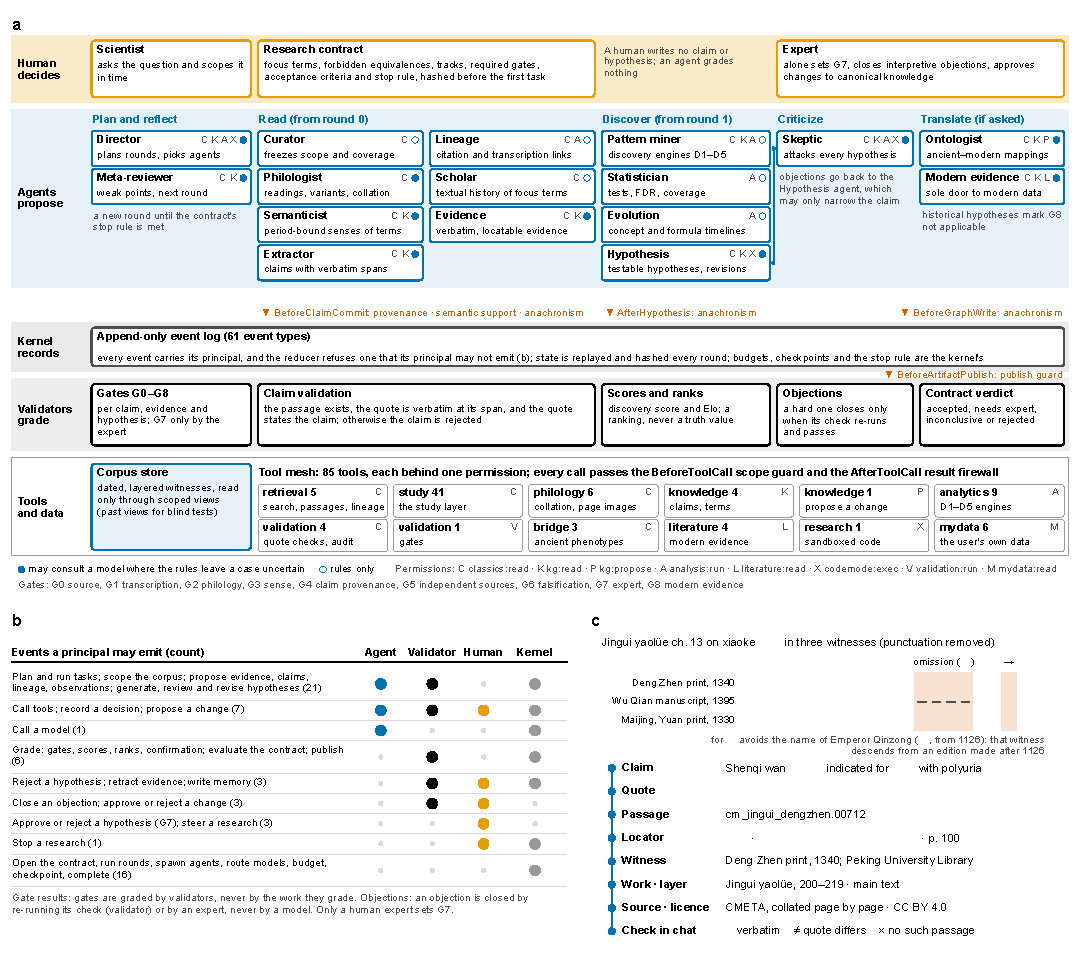
\includegraphics[width=1\textwidth,height=\textheight]{../../../figures/out/fig1_architecture.pdf}

\textbf{Fig. 1.} TaoChronos: agents propose, validators grade, experts
decide. (a) The agent by principal (rows) and stage of a research round
(columns); letters, permissions; filled circles, agents that may consult
a model; vermilion, the hooks; validators alone grade, and only the
expert sets G7. (b) Event authority: which principals may emit each
group of the 61 event types. (c) One clause of the \emph{Jingui yaolüe}
in three witnesses aligned character by character, with the provenance
chain of one witness from claim to license.

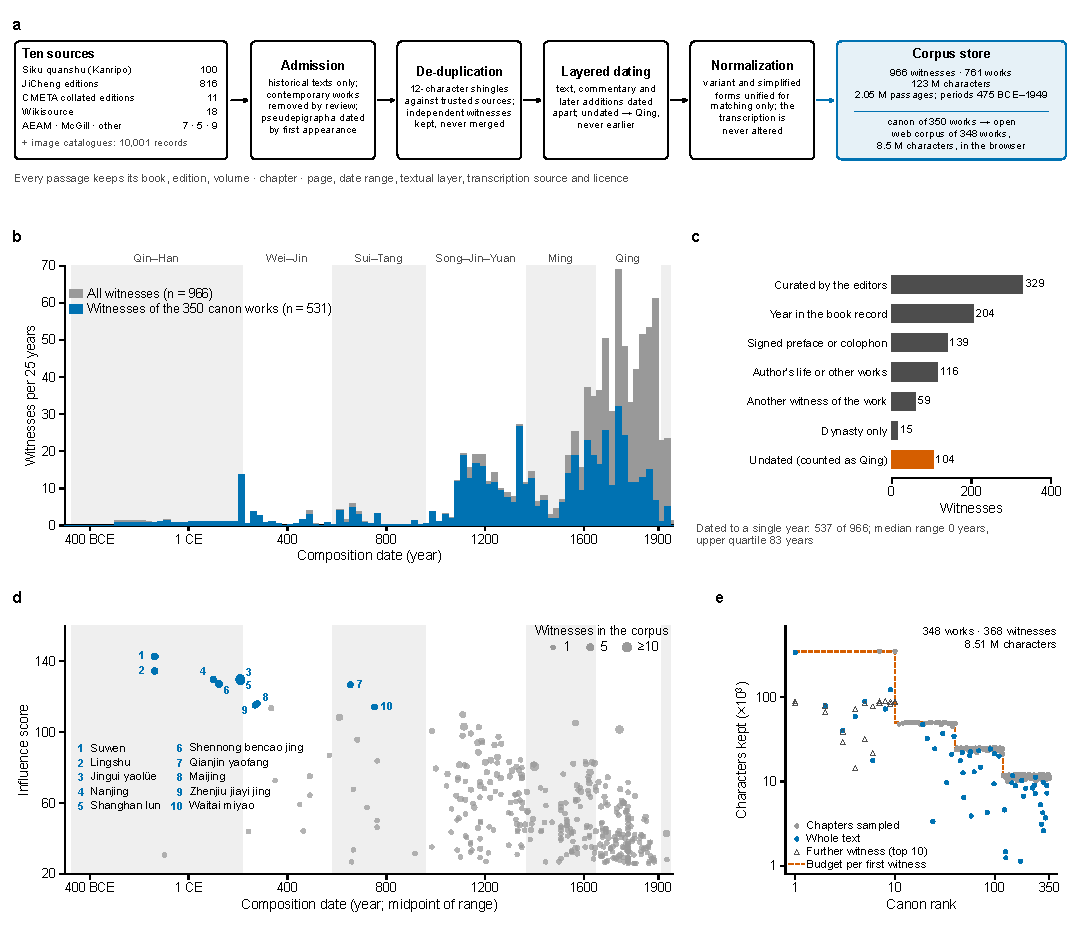
\includegraphics[width=1\textwidth,height=\textheight]{../../../figures/out/fig2_corpus.pdf}

\textbf{Fig. 2.} The corpus. (a) Construction from ten sources. (b)
Witnesses per 25-year bin (n = 966; blue, the 531 witnesses of the 350
canon works). (c) Basis of dating; undated witnesses counted as Qing.
(d) Influence score of the canon works against composition date. (e)
Characters kept per witness of the open web corpus against canon rank.

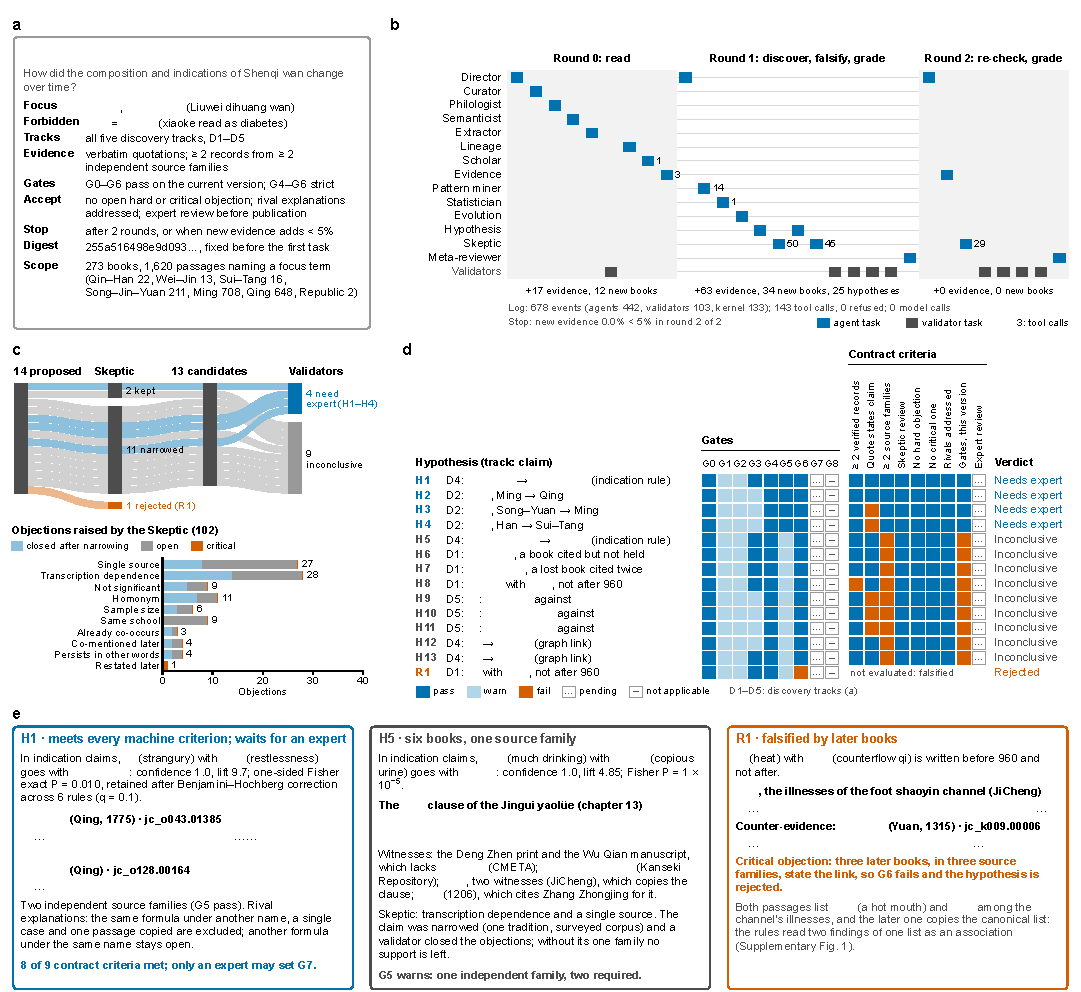
\includegraphics[width=1\textwidth,height=\textheight]{../../../figures/out/fig3_end_to_end.pdf}

\textbf{Fig. 3.} One research question end to end (rules only). (a)
Question and contract. (b) The 30 tasks by round and agent; numbers,
tool calls. (c) The 14 hypotheses through the Skeptic and the
validators, and the 117 objections by check. (d) Final hypotheses
against gates and contract criteria. (e) Three outcomes with verbatim
evidence. D1--D5, discovery tracks.

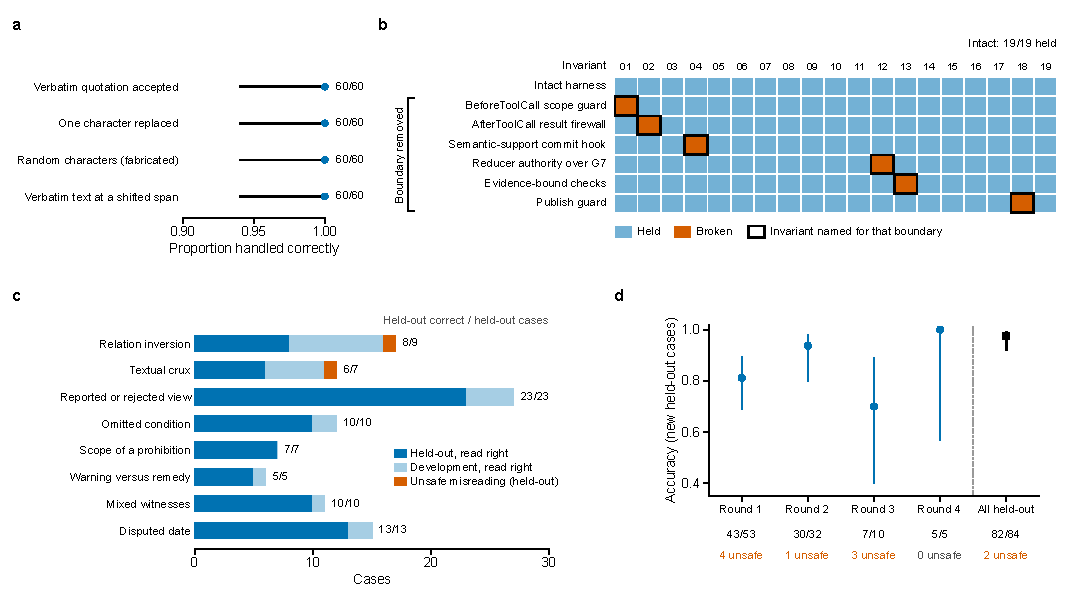
\includegraphics[width=1\textwidth,height=\textheight]{../../../figures/out/fig4_verification.pdf}

\textbf{Fig. 4.} Verification and safety. (a) Quotation checks on 60
random passages; lines, Wilson 95\% CIs. (b) Nineteen invariants on the
intact agent and six variants with one boundary removed each (outlined,
the invariant named for that boundary). (c) 107 hard interpretive cases
in eight classes; numbers, held-out correct. (d) Accuracy in four blind
rounds and on all held-out cases; lines, Wilson 95\% CIs.

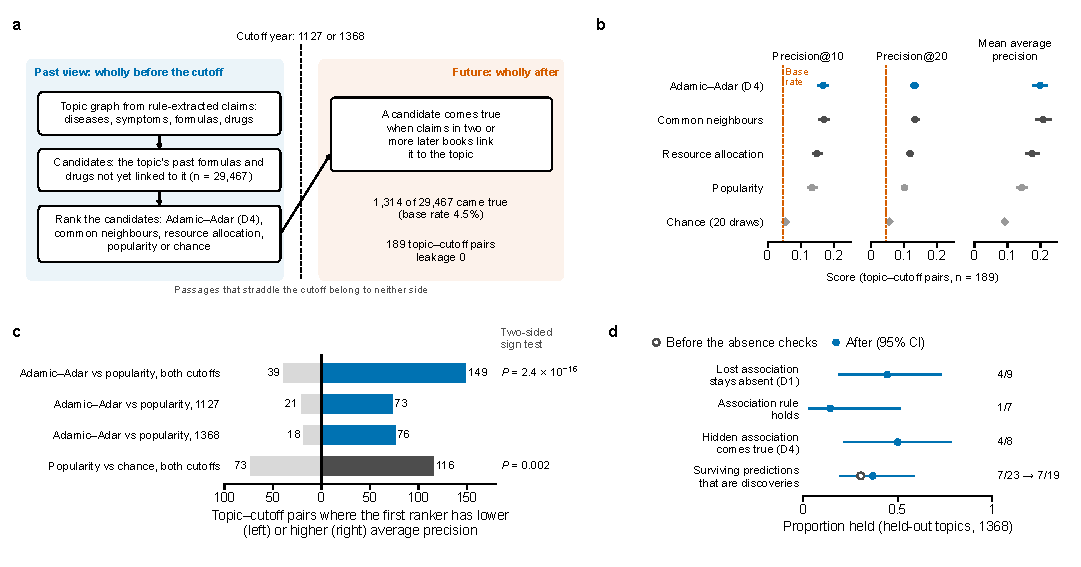
\includegraphics[width=1\textwidth,height=\textheight]{../../../figures/out/fig5_research_value.pdf}

\textbf{Fig. 5.} Research value. (a) The blind temporal benchmark. (b)
Precision at 10 and 20 and mean average precision of five rankers over
189 topic--cutoff pairs (95\% CIs). (c) Paired comparisons of average
precision, two-sided sign tests. (d) Predictions of the whole pipeline
at 1368 on four held-out topics borne out by later books (Wilson 95\%
CIs).

\textbf{Table 1 \textbar{} Eight ways an agent can go wrong on the
classical literature, the mechanism that stops each in TaoChronos, and
the measured evidence that it does}

\begin{longtable}[]{@{}
  >{\raggedright\arraybackslash}p{(\columnwidth - 6\tabcolsep) * \real{0.2500}}
  >{\raggedright\arraybackslash}p{(\columnwidth - 6\tabcolsep) * \real{0.2500}}
  >{\raggedright\arraybackslash}p{(\columnwidth - 6\tabcolsep) * \real{0.2500}}
  >{\raggedright\arraybackslash}p{(\columnwidth - 6\tabcolsep) * \real{0.2500}}@{}}
\toprule\noalign{}
\begin{minipage}[b]{\linewidth}\raggedright
Failure mode
\end{minipage} & \begin{minipage}[b]{\linewidth}\raggedright
Example in the classics
\end{minipage} & \begin{minipage}[b]{\linewidth}\raggedright
Mechanism in TaoChronos
\end{minipage} & \begin{minipage}[b]{\linewidth}\raggedright
Evidence in this study
\end{minipage} \\
\midrule\noalign{}
\endhead
\bottomrule\noalign{}
\endlastfoot
Fabricated or altered quotation & A quote with one character changed, or
the right words at the wrong place & The harness, not the producer,
locates every quote in its passage at commit (verbatim, or after
length-preserving variant normalization); the conversation client checks
every cited passage & 180/180 corrupted quotations rejected, 60/60
verbatim accepted; 100\% of committed claims verbatim (Fig. 4a) \\
True quote, false reading & 「不可发汗，宜桂枝汤」 (a prohibition beside
a prescription); 「或曰\ldots 余曰非也」 (a view the author rejects) &
Semantic-support hook reads each claim's statement frame (speaker,
stance, conditions, negations) and refuses a claim its quote
contradicts; a registry of textual cruxes harvested from commentaries
makes doubtful clauses read as ambiguous & Held-out hard cases 82/84, 2
unsafe; four blind rounds (Fig. 4c,d) \\
Copies counted as independent testimony & Five witnesses of one clause
of the Jingui yaolüe and its copy in the Maijing & Gate G5 counts
independent source families (author and transcription clusters), not
books; the Skeptic checks transcription dependence and single sources &
H2 held inconclusive on one family (Fig. 3e); an over-merging of
families reported (Supplementary Fig. 1) \\
Anachronism (presentism) & Xiaoke 消渴 read as diabetes mellitus;
shanghan 伤寒 read as typhoid & Anachronism guard at claim, hypothesis
and graph-write hooks; the contract's forbidden equivalences; the
ancient--modern bridge states phenotypic similarity with typed
relations, never a retrospective diagnosis & Statements 10/10, mappings
8/8, translations 24/24; agent-asserted equivalence blocked \\
Arguments from silence & An association called lost after 960 that a
later book still states & The Skeptic searches the whole scope for
explicit, supported statements; one later statement refutes a loss and
any statement refutes a hidden link, as hard, critical objections no
rewording can close & 2 wrong lost and 2 already-written hidden
associations rejected, and no discovery (Fig. 5d); R1 rejected (Fig.
3) \\
Self-grading and premature acceptance & A model closing its own
objection, setting expert approval, or a finished run taken as an
accepted finding & Every event carries its principal and the reducer
refuses an event its principal may not emit (61 types); only validators
grade, only a human sets G7; an executable contract judges acceptance &
19/19 invariants held; each of 6 boundaries removed broke its invariant
and no other (Fig. 4b) \\
Hindsight in testing foresight & A `prediction' made after reading the
books that later confirm it & Time-machine views bounded in SQL on every
read path; passages that straddle the cutoff belong to neither side;
leakage counted, not assumed & Leakage 0; precision@10 0.168 against
0.134 (popularity) and 0.054 (chance)† (Fig. 5) \\
Irreproducible runs & A result that cannot be rerun or audited step by
step & Append-only event log replayed and hashed every round; tool-call
receipts in a hash chain; recorded model responses replayed exactly &
Resume after a crash at 4 of 4 points reaches the same state; reruns and
parallel runs identical; the end-to-end report rewritten identically \\
\end{longtable}

Every mechanism is deterministic code that runs whether a language model
or a rule produced the output; all evidence was measured with the rules
alone (no model called).

†Needs the full corpus store, which is not distributed; values from
docs/evals.md. Other values were reproduced by \texttt{taochronos\ eval}
on the demonstration corpus.

\hypertarget{acknowledgments}{%
\section*{Acknowledgments}\label{acknowledgments}}
\addcontentsline{toc}{section}{Acknowledgments}

We thank the editors and volunteers of the Kanseki Repository, 中醫笈成,
數位中醫校書郎 CMETA, Wikisource, McGill University Library and the Tōa
Igaku Kyōkai. {[}Funding: grant numbers.{]}

\hypertarget{compliance-with-ethics-guidelines}{%
\section*{Compliance with ethics
guidelines}\label{compliance-with-ethics-guidelines}}
\addcontentsline{toc}{section}{Compliance with ethics guidelines}

{[}Author names{]} declare that they have no conflict of interest or
financial conflicts to disclose. {[}Amend: IMPF-AI operates the web
deployment of TaoChronos; declare any relationship with ZhongJingGPT.{]}
No human or animal subjects were involved; the real-world-data path was
tested on a synthetic database only.

\hypertarget{credit-authorship-contribution-statement}{%
\section*{CRediT authorship contribution
statement}\label{credit-authorship-contribution-statement}}
\addcontentsline{toc}{section}{CRediT authorship contribution statement}

{[}Author 1{]}: Conceptualization, Software, Methodology, Writing --
original draft. {[}Author 2{]}: Data curation, Validation, Writing --
review \& editing. {[}To be completed.{]}

\hypertarget{declaration-of-generative-ai-and-ai-assisted-technologies-in-the-writing-process}{%
\section*{Declaration of generative AI and AI-assisted technologies in
the writing
process}\label{declaration-of-generative-ai-and-ai-assisted-technologies-in-the-writing-process}}
\addcontentsline{toc}{section}{Declaration of generative AI and
AI-assisted technologies in the writing process}

{[}Declare here, as the journal requires, any use of generative AI in
preparing this manuscript. No language model was called in any analysis
reported in this paper.{]}

\hypertarget{data-and-code-availability}{%
\section*{Data and code availability}\label{data-and-code-availability}}
\addcontentsline{toc}{section}{Data and code availability}

Code, the open canon corpus, source catalogs with licenses, evaluation
gold sets and the source data of every figure are at
\url{https://github.com/psknlr/TaoChronos} ({[}license{]}; version
{[}tag/commit{]}). The full corpus store is not redistributed because
some sources forbid redistribution; it is rebuilt from the pinned
sources (\texttt{docs/data.md}).

\hypertarget{appendix-a.-supplementary-data}{%
\section*{Appendix A. Supplementary
data}\label{appendix-a.-supplementary-data}}
\addcontentsline{toc}{section}{Appendix A. Supplementary data}

Supplementary data to this article (Supplementary Notes 1--4,
Supplementary Figs. 1--5, Supplementary Tables 1--14 and Supplementary
Data 1--2) can be found online.

\hypertarget{references}{%
\section*{References}\label{references}}
\addcontentsline{toc}{section}{References}

\hypertarget{refs}{}
\begin{CSLReferences}{0}{0}
\leavevmode\vadjust pre{\hypertarget{ref-tu2011artemisinin}{}}%
\CSLLeftMargin{{[}1{]} }%
\CSLRightInline{Tu Y. The discovery of artemisinin (qinghaosu) and gifts
from {Chinese} medicine. Nature Medicine 2011;17:1217--20.
\url{https://doi.org/10.1038/nm.2471}.}

\leavevmode\vadjust pre{\hypertarget{ref-wang2008apl}{}}%
\CSLLeftMargin{{[}2{]} }%
\CSLRightInline{Wang Z-Y, Chen Z. Acute promyelocytic leukemia: From
highly fatal to highly curable. Blood 2008;111:2505--15.
\url{https://doi.org/10.1182/blood-2007-07-102798}.}

\leavevmode\vadjust pre{\hypertarget{ref-swanson1986fish}{}}%
\CSLLeftMargin{{[}3{]} }%
\CSLRightInline{Swanson DR. Fish oil, {Raynaud's} syndrome, and
undiscovered public knowledge. Perspectives in Biology and Medicine
1986;30:7--18. \url{https://doi.org/10.1353/pbm.1986.0087}.}

\leavevmode\vadjust pre{\hypertarget{ref-tshitoyan2019unsupervised}{}}%
\CSLLeftMargin{{[}4{]} }%
\CSLRightInline{Tshitoyan V, Dagdelen J, Weston L, Dunn A, Rong Z,
Kononova O, et al. Unsupervised word embeddings capture latent knowledge
from materials science literature. Nature 2019;571:95--8.
\url{https://doi.org/10.1038/s41586-019-1335-8}.}

\leavevmode\vadjust pre{\hypertarget{ref-krenn2023forecasting}{}}%
\CSLLeftMargin{{[}5{]} }%
\CSLRightInline{Krenn M et al. Forecasting the future of artificial
intelligence with machine learning-based link prediction in an
exponentially growing knowledge network. Nature Machine Intelligence
2023;5:1326--35. \url{https://doi.org/10.1038/s42256-023-00735-0}.}

\leavevmode\vadjust pre{\hypertarget{ref-kang2025zhongjinggpt}{}}%
\CSLLeftMargin{{[}6{]} }%
\CSLRightInline{Kang Y, Chang Y, Wu S, Wu X, Jiao Y, Fu J, et al.
{ZhongJingGPT}: An expert knowledge-guided language model for
traditional {Chinese} medicine. Tsinghua Science and Technology 2025.
\url{https://doi.org/10.26599/TST.2025.9010046}.}

\leavevmode\vadjust pre{\hypertarget{ref-cmlm2023zhongjing}{}}%
\CSLLeftMargin{{[}7{]} }%
\CSLRightInline{CMLM-ZhongJing team.
\href{https://github.com/pariskang/CMLM-ZhongJing}{{CMLM-ZhongJing}: The
first-ever traditional {Chinese} medicine large language model} 2023.}

\leavevmode\vadjust pre{\hypertarget{ref-zhang2023huatuogpt}{}}%
\CSLLeftMargin{{[}8{]} }%
\CSLRightInline{Zhang H, Chen J, Jiang F, et al.
\href{https://aclanthology.org/2023.findings-emnlp.725}{{HuatuoGPT},
towards taming language model to be a doctor}. Findings of the
association for computational linguistics: EMNLP 2023, 2023, p.
10859--85.}

\leavevmode\vadjust pre{\hypertarget{ref-yang2024zhongjing}{}}%
\CSLLeftMargin{{[}9{]} }%
\CSLRightInline{Yang S, Zhao H, Zhu S, Zhou G, Xu H, Jia Y, et al.
Zhongjing: Enhancing the {Chinese} medical capabilities of large
language model through expert feedback and real-world multi-turn
dialogue. Proceedings of the AAAI conference on artificial intelligence,
vol. 38, 2024. \url{https://doi.org/10.1609/aaai.v38i17.29907}.}

\leavevmode\vadjust pre{\hypertarget{ref-yue2024tcmbench}{}}%
\CSLLeftMargin{{[}10{]} }%
\CSLRightInline{Yue W, Wang X, Zhu W, Guan M, Zheng H, Wang P, et al.
{TCMBench}: A comprehensive benchmark for evaluating large language
models in traditional {Chinese} medicine 2024.
\url{https://doi.org/10.48550/arXiv.2406.01126}.}

\leavevmode\vadjust pre{\hypertarget{ref-li2025tcmrdkg}{}}%
\CSLLeftMargin{{[}11{]} }%
\CSLRightInline{Li H, Xia C, Hou Y, Hu S, Liu Y, Jiang Q. {TCMRD-KG}:
Innovative design and development of rheumatology knowledge graph in
ancient {Chinese} literature assisted by large language models.
Frontiers in Pharmacology 2025;16:1535596.
\url{https://doi.org/10.3389/fphar.2025.1535596}.}

\leavevmode\vadjust pre{\hypertarget{ref-xiang2025kgclassics}{}}%
\CSLLeftMargin{{[}12{]} }%
\CSLRightInline{Xiang S, Lin H, Cai F, Jiang Z. Integrating knowledge
graphs with ancient {Chinese} medicine classics: Challenges and future
prospects of multi-agent system convergence. Chinese Medicine 2025.
\url{https://doi.org/10.1186/s13020-025-01226-7}.}

\leavevmode\vadjust pre{\hypertarget{ref-boiko2023autonomous}{}}%
\CSLLeftMargin{{[}13{]} }%
\CSLRightInline{Boiko DA, MacKnight R, Kline B, Gomes G. Autonomous
chemical research with large language models. Nature 2023;624:570--8.
\url{https://doi.org/10.1038/s41586-023-06792-0}.}

\leavevmode\vadjust pre{\hypertarget{ref-gottweis2025coscientist}{}}%
\CSLLeftMargin{{[}14{]} }%
\CSLRightInline{Gottweis J et al. Towards an {AI} co-scientist 2025.
\url{https://doi.org/10.48550/arXiv.2502.18864}.}

\leavevmode\vadjust pre{\hypertarget{ref-swanson2025virtuallab}{}}%
\CSLLeftMargin{{[}15{]} }%
\CSLRightInline{Swanson K, Wu W, Bulaong NL, Pak JE, Zou J. The {Virtual
Lab} of {AI} agents designs new {SARS-CoV-2} nanobodies. Nature
2025;646:716--23. \url{https://doi.org/10.1038/s41586-025-09442-9}.}

\leavevmode\vadjust pre{\hypertarget{ref-huang2025popper}{}}%
\CSLLeftMargin{{[}16{]} }%
\CSLRightInline{Huang K, Jin Y, Li R, Li MY, Candès E, Leskovec J.
\href{https://proceedings.mlr.press/v267/huang25n.html}{Automated
hypothesis validation with agentic sequential falsifications}.
Proceedings of the 42nd international conference on machine learning,
vol. 267, 2025, p. 25372--437.}

\leavevmode\vadjust pre{\hypertarget{ref-lu2026endtoend}{}}%
\CSLLeftMargin{{[}17{]} }%
\CSLRightInline{Lu C, Lu C, Lange RT, Yamada Y, Hu S, Foerster J, et al.
Towards end-to-end automation of {AI} research. Nature 2026;651:914--9.
\url{https://doi.org/10.1038/s41586-026-10265-5}.}

\leavevmode\vadjust pre{\hypertarget{ref-ji2023hallucination}{}}%
\CSLLeftMargin{{[}18{]} }%
\CSLRightInline{Ji Z, Lee N, Frieske R, Yu T, Su D, Xu Y, et al. Survey
of hallucination in natural language generation. ACM Computing Surveys
2023;55:1--38. \url{https://doi.org/10.1145/3571730}.}

\leavevmode\vadjust pre{\hypertarget{ref-gao2023alce}{}}%
\CSLLeftMargin{{[}19{]} }%
\CSLRightInline{Gao T, Yen H, Yu J, Chen D. Enabling large language
models to generate text with citations. Proceedings of the 2023
conference on empirical methods in natural language processing, 2023, p.
6465--88. \url{https://doi.org/10.18653/v1/2023.emnlp-main.398}.}

\leavevmode\vadjust pre{\hypertarget{ref-thirunavukarasu2023llm}{}}%
\CSLLeftMargin{{[}20{]} }%
\CSLRightInline{Thirunavukarasu AJ, Ting DSJ, Elangovan K, Gutierrez L,
Tan TF, Ting DSW. Large language models in medicine. Nature Medicine
2023;29:1930--40. \url{https://doi.org/10.1038/s41591-023-02448-8}.}

\leavevmode\vadjust pre{\hypertarget{ref-kohler2021hpo}{}}%
\CSLLeftMargin{{[}21{]} }%
\CSLRightInline{Köhler S et al. The {Human Phenotype Ontology} in 2021.
Nucleic Acids Research 2021;49:D1207--17.
\url{https://doi.org/10.1093/nar/gkaa1043}.}

\leavevmode\vadjust pre{\hypertarget{ref-adamic2003friends}{}}%
\CSLLeftMargin{{[}22{]} }%
\CSLRightInline{Adamic LA, Adar E. Friends and neighbors on the {Web}.
Social Networks 2003;25:211--30.
\url{https://doi.org/10.1016/S0378-8733(03)00009-1}.}

\leavevmode\vadjust pre{\hypertarget{ref-popper1959logic}{}}%
\CSLLeftMargin{{[}23{]} }%
\CSLRightInline{Popper KR. The logic of scientific discovery. London:
Hutchinson; 1959.}

\leavevmode\vadjust pre{\hypertarget{ref-jia2011mutation}{}}%
\CSLLeftMargin{{[}24{]} }%
\CSLRightInline{Jia Y, Harman M. An analysis and survey of the
development of mutation testing. IEEE Transactions on Software
Engineering 2011;37:649--78. \url{https://doi.org/10.1109/TSE.2010.62}.}

\leavevmode\vadjust pre{\hypertarget{ref-wilson1927probable}{}}%
\CSLLeftMargin{{[}25{]} }%
\CSLRightInline{Wilson EB. Probable inference, the law of succession,
and statistical inference. Journal of the American Statistical
Association 1927;22:209--12.
\url{https://doi.org/10.1080/01621459.1927.10502953}.}

\leavevmode\vadjust pre{\hypertarget{ref-armitage1955tests}{}}%
\CSLLeftMargin{{[}26{]} }%
\CSLRightInline{Armitage P. Tests for linear trends in proportions and
frequencies. Biometrics 1955;11:375--86.
\url{https://doi.org/10.2307/3001775}.}

\leavevmode\vadjust pre{\hypertarget{ref-hripcsak2015ohdsi}{}}%
\CSLLeftMargin{{[}27{]} }%
\CSLRightInline{Hripcsak G et al. Observational {Health Data Sciences
and Informatics} ({OHDSI}): Opportunities for observational researchers.
Studies in Health Technology and Informatics 2015;216:574--8.
\url{https://doi.org/10.3233/978-1-61499-564-7-574}.}

\leavevmode\vadjust pre{\hypertarget{ref-libennowell2007link}{}}%
\CSLLeftMargin{{[}28{]} }%
\CSLRightInline{Liben-Nowell D, Kleinberg J. The link-prediction problem
for social networks. Journal of the American Society for Information
Science and Technology 2007;58:1019--31.
\url{https://doi.org/10.1002/asi.20591}.}

\end{CSLReferences}

\end{document}
